\chapter{Experimento: ¿Dos códigos de test parecidos prueban lo mismo? }\aplabel{exp-static-vs-dynamic}

\par Uno de los primeras actividades al enfrentar el problema de modularidad de los test es mirar el código fuente. Luego de una breve y ligera inspección podemos encontrar varios tests similares que difieren en pocas líneas de código lo cual motiva distintas estrategias de refactorización~\cite{roy2007survey,rattan2013software,Kosc13a}. Sin embargo, surge la siguiente interrogante, ¿En qué afecta esto en la cobertura de estos tests? Es más, la pregunta motiva ir un paso atrás, si estos dos tests son similares en su código, ¿cubren los mismos métodos?.

\par De esta pregunta se desprenden dos enfoques para analizar similtud de test: estático y dinamico. En el análisis estático para determinar similitud en el código fuente, y en el dinámico qué tan similar es su cobertura~\cite{Horwi02a} lo cual solo se puede determinar analizado su ejecución. Para responder esta pregunta se realizó un experimento que compara la correlación entre dos métricas que apuntan a comparar las pruebas de software desde estos dos aspectos.

\section{Metodología}

\par El experimento consta entonces de verificar si existe o no correlación  entre la similitud de código (o \emph{estática}) y la similitud de ejecución (o \emph{dinámica}). Para ello se escogió dos métricas de similitud, una por cada acercamiento al problema, y se realizó comparaciones entre todos los tests de todos los unit tests de un software. Este experimento se realizó sobre los unit tests de 2 softwares con propósitos muy distintos. Estos son: 

\begin{enumerate} 
\item \emph{Roassal}\footnote{Para mayor información, ver \secref{caso-estudio-roassal}}: Motor de visualización ágil.
\item \emph{Fuel}\footnote{RMoD . Fuel [en línea] \textless\url{http://rmod.lille.inria.fr/web/pier/software/Fuel}\textgreater [Consulta: 12/08/2013] }: Framework de serialización de objetos desarrollado en Pharo.
%\item \emph{Network}\footnote{Network es parte del núcleo de la plataforma Pharo - \url{http://www.pharo-project.org}}: Componente de la plataforma Pharo relacionado a redes y comunicación (sockets, protocolos de red, etc).
\end{enumerate}

\par El experimento fue implementado y ejecutado en la plataforma Pharo. Además las aplicaciones previamente descritas fueron seleccionadas pues ya han sido utilizadas en trabajos previos~\cite{Berg11d}.

\subsection{Métricas de similitud}\seclabel{exp1-metricas-sim}
\par Para esto, se realizó un experimento que compara la similitud estática y dinámica de los test. Las métrica de similitud escogidas fueron normalizadas para obtener valores entre $\left[ 0 , 1 \right]$. Un valor muy cercano a $0$ significa que los elementos son poco similares o muy diferentes, y por su parte, un valor muy cerano a 1 indica que los elementos son muy parecidos. 

% 0<delta(tr,tb)<1 --> $0\leq \delta(t_r,t_b) \leq 1$
\par La \emph{métrica de similitud estática}, $f(t_a,t_b)$, compara el código de los test según el número de líneas que tienen en común contra el total de líneas entre ambos (sin contar dos veces líneas en común). Entre las líneas de un método no se contó la primera línea (firma del método) ni sus líneas en blanco. Formalmente, sea $L_{a}$ el conjunto de líneas que componen el código del test $t_a$ y  $L_{b}$ de $t_b$ respectivamente, $f$ se define como: 

\[ f(t_a,t_b)= \dfrac{\abs{L_{a} \cap L_{b}}}{\abs{L_{a} \cup L_{b}}} , \quad f(t_a,t_b) \in \left[ 0 , 1 \right] \]

\par La \emph{métrica de similitud dinámica}, $g(t_a,t_b)$, por su parte, compara la cobertura de cada test según los métodos del código base que fueron testeados. Es decir, los métodos ejecutados en común contra el total de métodos llamados durante la ejecución de ambos métodos. Formalmente, sea $T_{a}$ el conjunto de métodos llamados durante la ejecución del test $t_a$ y $T_{b}$ el correspondiente a $t_b$, $g$ se define como: 

\[ g(t_a,t_b)= \dfrac{\abs{T_{a} \cap T_{b}}}{\abs{T_{a} \cup T_{b}}} , \quad g(t_a,t_b) \in \left[ 0 , 1 \right] \]


\section{Resultados y Conclusiones}

\par Luego de realizar el experimentos en los dos softwares mencionados, los resultados se presentan en los gráficos de puntos (o scatterplot) de la \figref{ap-stat-dyn}, donde cada punto en el gráfico corresponde a un par ($f(t_a,t_b),g(t_a,t_b)$).

\begin{figure}
\centering

\begin{tabular}{c}
\subfloat[Roassal - $\rho_{f,g}=0,1572$]{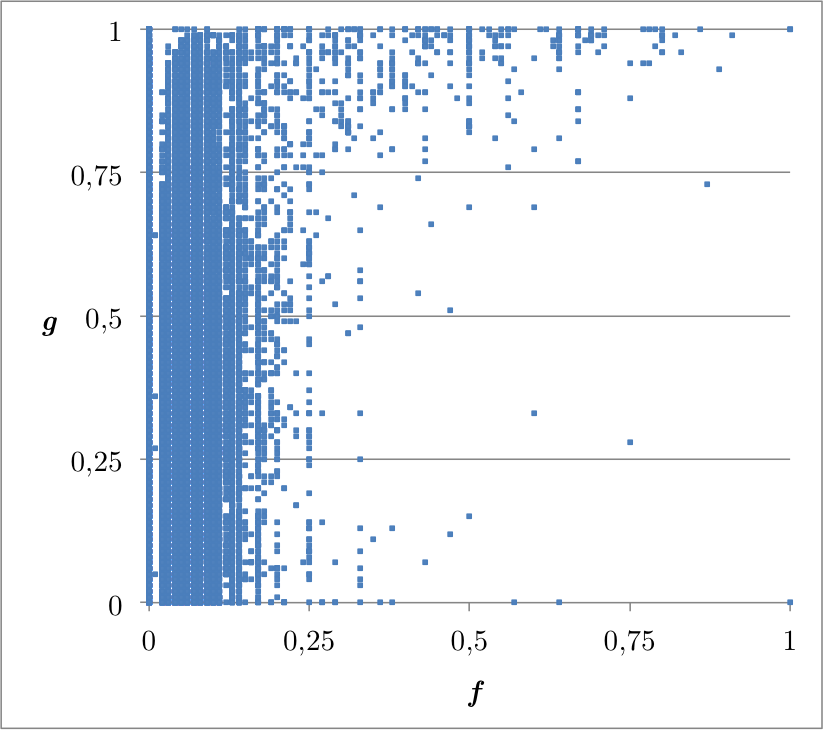
\includegraphics[width=8cm]{images/ap-staticvsdynamic/roassal.png}} \\[2cm] 
\subfloat[Fuel - $\rho_{f,g}=0,1176$]{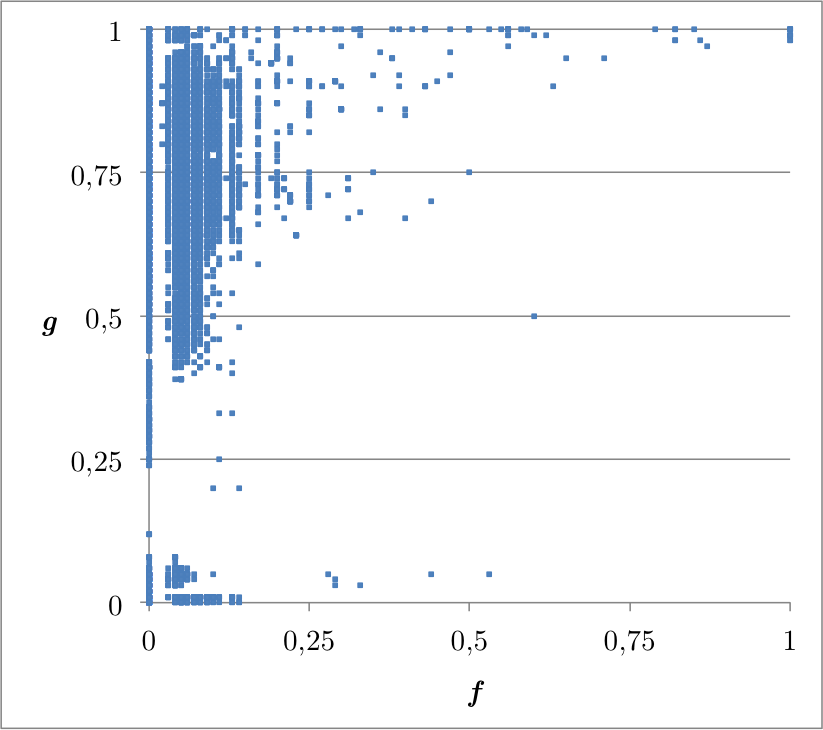
\includegraphics[width=8cm]{images/ap-staticvsdynamic/fuel.png}}
\end{tabular}
\caption{Resultados comparación de métricas $f$ y $g$}
\figlabel{ap-stat-dyn}
\end{figure}

\par Los graficos muestran que no existe correlación entre las dos métricas ya que en ninguno de los gráficos se ve alguna forma linear que lo indique. Esto último se ve reforzado cuando se toma en cuenta los valores del coeficiente de correlación de Pearson ($\rho_{f,g}$) de cada uno que son muy cercanos a cero, lo que indica que no existe correlación lineal entre las dos métricas.

\par Como consecuencia se puede deducir que dos tests con una gran porción de código duplicado no necesariamente tienen cubren los mismos métodos, o sea, no necesariamente testean la misma porción de código.

\par Se concluye que la duplicación de código entre tests no puede ser usado para inferir que son semánticamente similares. Por tanto, cualquier análisis comparativo entre tests debe hacerse considerando el código fuente y características de análsis estático, como también datos obtenidos durante su ejecución entre otros aspectos del análisis dinámico. 




%=====
%=====
%=====

% \par Para ilustrar lo anterior, se presenta el código de los tests: {\tt testAddingColoredElement} y {\tt testVisualizingBigClasses} 
% %=== Ejemplo
% \begin{codeWithLineNumbers}
% <i>testAddingColoredElement</i>
% 	canvas := ROView new.
% 	el1 := ROBox green element.
% 	el2 := ROBox red element.
% 	canvas add: el1; add: el2.
% 	self shouldnt: [ canvas open ] raise: Error

% <i>testVisualizingBigClasses</i>
% 	canvas := ROView new.
% 	Collection withAllSubclasses do: [ :cls |
% 		cls numberOfMethods > 10
% 			ifTrue: [ el := ROBox red element ]
% 			ifFalse: [ el := ROBox green element ].
% 		canvas add: el ].
% 	self shouldnt: [ canvas open ] raise: Error
% \end{codeWithLineNumbers}\codelabel{ejemplo-stat-dyn} 

% \par El código de {\tt testAddingColoredElement} crea un canvas (lienzo donde se dibujan los elementos gráficos) para posionar sobre esta una caja verde y otra roja. Por su parte, en {\tt testVisualizingBigClasses} se crea una visualizacion que representa algunas clases coloreadas según una condición particular. Cada subclase de {\tt Collection} está asociada a una caja. Si la clase tiene más de 10 métodos, la caja se pinta en rojo, de lo contrario en verde. 

% \par Los dos tests tienen un 95\% de metodos testeados en común, el 5\% que los diferencia se debe a algunos cachés están activados cuando el número de cajas excede cierto número límite. 
